\documentclass[11pt,a4paper]{article}
\usepackage[utf8]{inputenc}
\usepackage[spanish]{babel}
\usepackage{amsmath}
\usepackage{amsfonts}
\usepackage{amssymb}
\usepackage{graphicx}
\usepackage{float}

\author{Víctor Iranzo}
\title{Capítulo 7: Pruebas}
\setlength{\parskip}{10pt}

\graphicspath{ {Cap7_Images/} }

\begin{document}
\maketitle

\section{Tipos de pruebas}

El siguiente esquema es una modificación del cuadrante de Marick  empleada para catalogar pruebas en distintos tipos:

\begin{figure}[h]
\centering
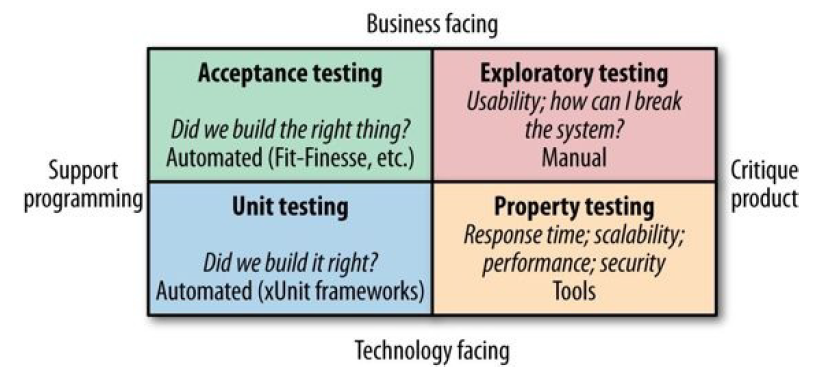
\includegraphics[scale=0.5]{Marick_Quadrant}
\caption{Modificación del cuadrante de Marick hecha por L.Crispin y J.Gregory en su libro Agile Testing.}
\end{figure}

Las pruebas situadas en la mitad inferior están relacionadas con la tecnología empleada, como son las pruebas unitarias o las de rendimiento, que deben ser implementadas por los desarrolladores y que se pueden automatizar. Las pruebas situadas en la mitad superior están orientadas a que los stakeholders conozcan cómo funciona el sistema y que no guardan relación con aspectos tecnológicos. Entran dentro de esta mitad las pruebas de aceptación o las pruebas manuales.

La proporción necesaria de cada tipo de test depende del sistema a desarrollar. La tendencia actual es en favor de los tests de pequeña escala y automatizados. En un sistema basado en microservicios, son esenciales las pruebas de este tipo ya que validarán que no se despliegue a producción código defectuoso.

Podemos clasificar las pruebas en los microservicios en 3 tipos según su alcance: unitarias, de servicios y de extremo a extremo. Estos términos pueden llevar a discusión: por ejemplo, en una prueba unitarias se puede incluir para algunas personas la validación de diferentes clases o funciones mientras que para otras no.

\begin{figure}[h]
\centering
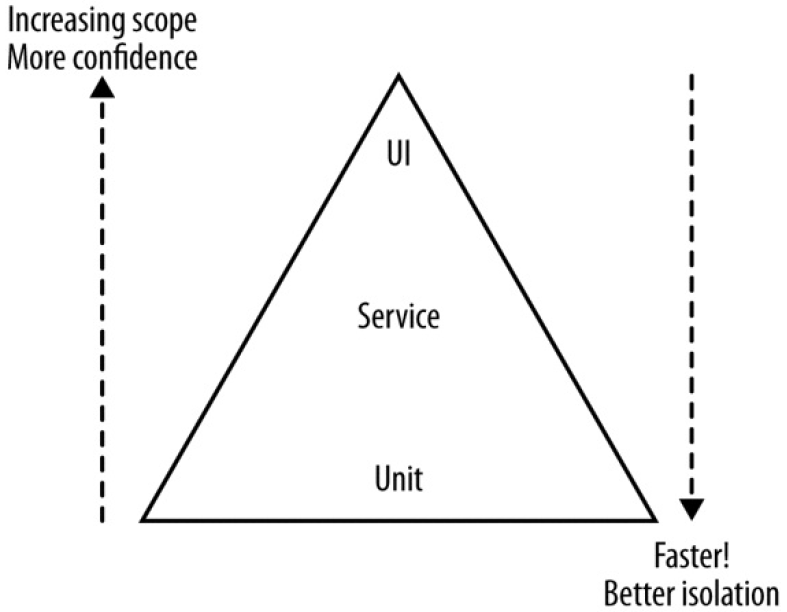
\includegraphics[scale=0.5]{Cohn_Pyramid}
\caption{Pirámide de pruebas diseñada por Mike Cohn en su libro Succeding with Agile.}
\end{figure}


\subsection{Pruebas unitarias}

Son pruebas que validan una única función. Se pueden generar fruto de procesos de desarrollo como el test-driven development (TDD). En general, se prefiere tener un gran número de este tipo de pruebas por su rapidez, porque pueden ayudar a la refactorización del código y porque es donde mayor cantidad de defectos se suele capturar.

\begin{figure}[H]
\centering
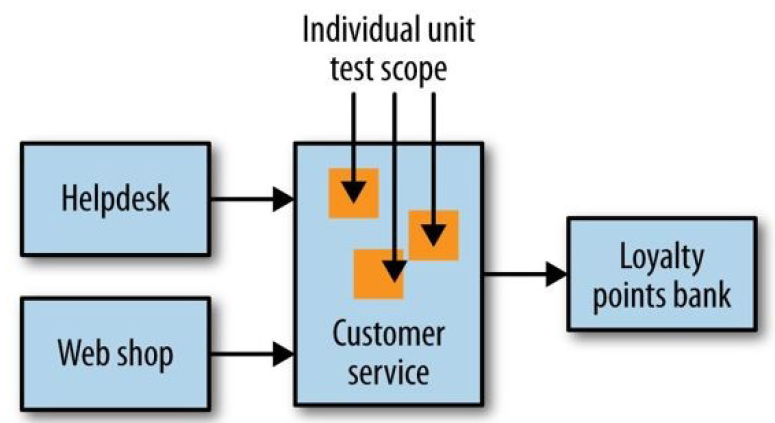
\includegraphics[scale=0.5]{Unit_Tests}
\caption{En las pruebas unitarias no se ejecuta ningún servicio, sino que se prueban métodos específicos de ellos.}
\end{figure}

\subsection{Pruebas de servicios}

En estas pruebas se verifica la funcionalidad de los servicios sin emplear las interfaces de usuario. Cada prueba verifica una de las funcionalidades que el servicio expone. Se pretende comprobar la separación entre los servicios y para solventar las dependencias que el servicio bajo pruebas tiene sobre otros, se reemplazan los servicios colaboradores por stubs o fakes.

Este tipo de pruebas pueden ser igual de rápidas que las unitarias siempre que no se tengan que emplear un gran número de infraestructuras como bases de datos o redes.

\begin{figure}[h]
\centering
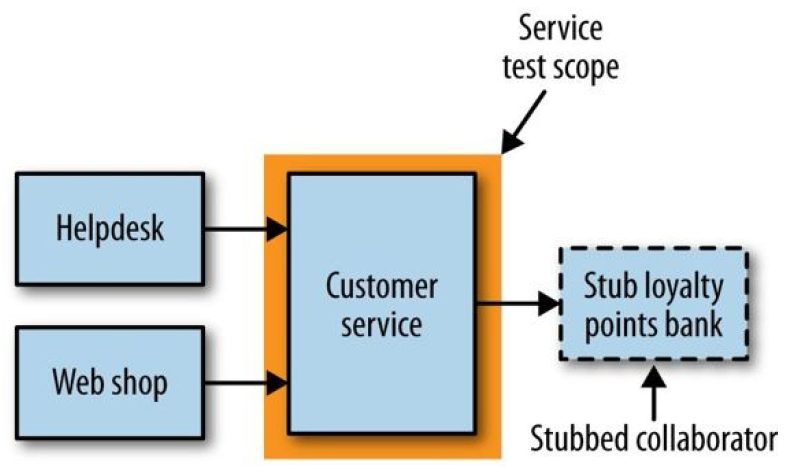
\includegraphics[scale=0.5]{Service_Tests}
\caption{Las pruebas de servicio se ejecutan sobre un único servicio y emplean fakes para reemplazar a los colaboradores de este.}
\end{figure}

\subsection{Pruebas de extremo a extremo}

Son pruebas que se ejecutan sobre todo el sistema. Cubren gran parte de código, por lo que su correcta ejecución dan mucho grado de confianza.

\begin{figure}[h]
\centering
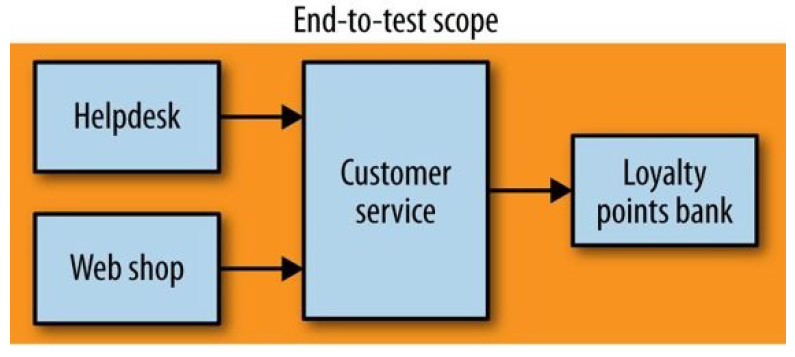
\includegraphics[scale=0.5]{End_To_End_Test}
\caption{Las pruebas de servicio se ejecutan sobre un único servicio y emplean fakes para reemplazar a los colaboradores de este.}
\end{figure}

\subsection{Pruebas dirigidas por el consumidor}

\section{Balance de pruebas a realizar}

\section{Pruebas frágiles y escamosas}

\section{Pruebas antes de producción}

\subsection{Despliegues verde y azul}

\subsection{Canary releases}

\subsection{Tiempo medio entre fallos y tiempo medio entre reparaciones}

\section{Pruebas de requisitos no funcionales}

\subsection{Pruebas de rendimiento}

\end{document}